% Options for packages loaded elsewhere
\PassOptionsToPackage{unicode}{hyperref}
\PassOptionsToPackage{hyphens}{url}
%
\documentclass[
]{book}
\title{Vascular Surgery Board Review}
\author{Audible Bleeding}
\date{2022-01-22}

\usepackage{amsmath,amssymb}
\usepackage{lmodern}
\usepackage{iftex}
\ifPDFTeX
  \usepackage[T1]{fontenc}
  \usepackage[utf8]{inputenc}
  \usepackage{textcomp} % provide euro and other symbols
\else % if luatex or xetex
  \usepackage{unicode-math}
  \defaultfontfeatures{Scale=MatchLowercase}
  \defaultfontfeatures[\rmfamily]{Ligatures=TeX,Scale=1}
\fi
% Use upquote if available, for straight quotes in verbatim environments
\IfFileExists{upquote.sty}{\usepackage{upquote}}{}
\IfFileExists{microtype.sty}{% use microtype if available
  \usepackage[]{microtype}
  \UseMicrotypeSet[protrusion]{basicmath} % disable protrusion for tt fonts
}{}
\makeatletter
\@ifundefined{KOMAClassName}{% if non-KOMA class
  \IfFileExists{parskip.sty}{%
    \usepackage{parskip}
  }{% else
    \setlength{\parindent}{0pt}
    \setlength{\parskip}{6pt plus 2pt minus 1pt}}
}{% if KOMA class
  \KOMAoptions{parskip=half}}
\makeatother
\usepackage{xcolor}
\IfFileExists{xurl.sty}{\usepackage{xurl}}{} % add URL line breaks if available
\IfFileExists{bookmark.sty}{\usepackage{bookmark}}{\usepackage{hyperref}}
\hypersetup{
  pdftitle={Vascular Surgery Board Review},
  pdfauthor={Audible Bleeding},
  hidelinks,
  pdfcreator={LaTeX via pandoc}}
\urlstyle{same} % disable monospaced font for URLs
\usepackage{color}
\usepackage{fancyvrb}
\newcommand{\VerbBar}{|}
\newcommand{\VERB}{\Verb[commandchars=\\\{\}]}
\DefineVerbatimEnvironment{Highlighting}{Verbatim}{commandchars=\\\{\}}
% Add ',fontsize=\small' for more characters per line
\usepackage{framed}
\definecolor{shadecolor}{RGB}{248,248,248}
\newenvironment{Shaded}{\begin{snugshade}}{\end{snugshade}}
\newcommand{\AlertTok}[1]{\textcolor[rgb]{0.94,0.16,0.16}{#1}}
\newcommand{\AnnotationTok}[1]{\textcolor[rgb]{0.56,0.35,0.01}{\textbf{\textit{#1}}}}
\newcommand{\AttributeTok}[1]{\textcolor[rgb]{0.77,0.63,0.00}{#1}}
\newcommand{\BaseNTok}[1]{\textcolor[rgb]{0.00,0.00,0.81}{#1}}
\newcommand{\BuiltInTok}[1]{#1}
\newcommand{\CharTok}[1]{\textcolor[rgb]{0.31,0.60,0.02}{#1}}
\newcommand{\CommentTok}[1]{\textcolor[rgb]{0.56,0.35,0.01}{\textit{#1}}}
\newcommand{\CommentVarTok}[1]{\textcolor[rgb]{0.56,0.35,0.01}{\textbf{\textit{#1}}}}
\newcommand{\ConstantTok}[1]{\textcolor[rgb]{0.00,0.00,0.00}{#1}}
\newcommand{\ControlFlowTok}[1]{\textcolor[rgb]{0.13,0.29,0.53}{\textbf{#1}}}
\newcommand{\DataTypeTok}[1]{\textcolor[rgb]{0.13,0.29,0.53}{#1}}
\newcommand{\DecValTok}[1]{\textcolor[rgb]{0.00,0.00,0.81}{#1}}
\newcommand{\DocumentationTok}[1]{\textcolor[rgb]{0.56,0.35,0.01}{\textbf{\textit{#1}}}}
\newcommand{\ErrorTok}[1]{\textcolor[rgb]{0.64,0.00,0.00}{\textbf{#1}}}
\newcommand{\ExtensionTok}[1]{#1}
\newcommand{\FloatTok}[1]{\textcolor[rgb]{0.00,0.00,0.81}{#1}}
\newcommand{\FunctionTok}[1]{\textcolor[rgb]{0.00,0.00,0.00}{#1}}
\newcommand{\ImportTok}[1]{#1}
\newcommand{\InformationTok}[1]{\textcolor[rgb]{0.56,0.35,0.01}{\textbf{\textit{#1}}}}
\newcommand{\KeywordTok}[1]{\textcolor[rgb]{0.13,0.29,0.53}{\textbf{#1}}}
\newcommand{\NormalTok}[1]{#1}
\newcommand{\OperatorTok}[1]{\textcolor[rgb]{0.81,0.36,0.00}{\textbf{#1}}}
\newcommand{\OtherTok}[1]{\textcolor[rgb]{0.56,0.35,0.01}{#1}}
\newcommand{\PreprocessorTok}[1]{\textcolor[rgb]{0.56,0.35,0.01}{\textit{#1}}}
\newcommand{\RegionMarkerTok}[1]{#1}
\newcommand{\SpecialCharTok}[1]{\textcolor[rgb]{0.00,0.00,0.00}{#1}}
\newcommand{\SpecialStringTok}[1]{\textcolor[rgb]{0.31,0.60,0.02}{#1}}
\newcommand{\StringTok}[1]{\textcolor[rgb]{0.31,0.60,0.02}{#1}}
\newcommand{\VariableTok}[1]{\textcolor[rgb]{0.00,0.00,0.00}{#1}}
\newcommand{\VerbatimStringTok}[1]{\textcolor[rgb]{0.31,0.60,0.02}{#1}}
\newcommand{\WarningTok}[1]{\textcolor[rgb]{0.56,0.35,0.01}{\textbf{\textit{#1}}}}
\usepackage{longtable,booktabs,array}
\usepackage{calc} % for calculating minipage widths
% Correct order of tables after \paragraph or \subparagraph
\usepackage{etoolbox}
\makeatletter
\patchcmd\longtable{\par}{\if@noskipsec\mbox{}\fi\par}{}{}
\makeatother
% Allow footnotes in longtable head/foot
\IfFileExists{footnotehyper.sty}{\usepackage{footnotehyper}}{\usepackage{footnote}}
\makesavenoteenv{longtable}
\usepackage{graphicx}
\makeatletter
\def\maxwidth{\ifdim\Gin@nat@width>\linewidth\linewidth\else\Gin@nat@width\fi}
\def\maxheight{\ifdim\Gin@nat@height>\textheight\textheight\else\Gin@nat@height\fi}
\makeatother
% Scale images if necessary, so that they will not overflow the page
% margins by default, and it is still possible to overwrite the defaults
% using explicit options in \includegraphics[width, height, ...]{}
\setkeys{Gin}{width=\maxwidth,height=\maxheight,keepaspectratio}
% Set default figure placement to htbp
\makeatletter
\def\fps@figure{htbp}
\makeatother
\setlength{\emergencystretch}{3em} % prevent overfull lines
\providecommand{\tightlist}{%
  \setlength{\itemsep}{0pt}\setlength{\parskip}{0pt}}
\setcounter{secnumdepth}{5}
\usepackage{booktabs}
\ifLuaTeX
  \usepackage{selnolig}  % disable illegal ligatures
\fi
\usepackage[]{natbib}
\bibliographystyle{plainnat}

\usepackage{amsthm}
\newtheorem{theorem}{Theorem}[chapter]
\newtheorem{lemma}{Lemma}[chapter]
\newtheorem{corollary}{Corollary}[chapter]
\newtheorem{proposition}{Proposition}[chapter]
\newtheorem{conjecture}{Conjecture}[chapter]
\theoremstyle{definition}
\newtheorem{definition}{Definition}[chapter]
\theoremstyle{definition}
\newtheorem{example}{Example}[chapter]
\theoremstyle{definition}
\newtheorem{exercise}{Exercise}[chapter]
\theoremstyle{definition}
\newtheorem{hypothesis}{Hypothesis}[chapter]
\theoremstyle{remark}
\newtheorem*{remark}{Remark}
\newtheorem*{solution}{Solution}
\begin{document}
\maketitle

{
\setcounter{tocdepth}{1}
\tableofcontents
}
\hypertarget{about}{%
\chapter{About}\label{about}}

The content was developed here by the Audible Bleeding team to accompany our board review podcast episodes.

\hypertarget{usage}{%
\section{Usage}\label{usage}}

This is not a comprehensive guide but instead an outline of the most high yield information to help guide board preparation.\texttt{\{r\ include=FALSE\}\ \#\ automatically\ create\ a\ bib\ database\ for\ R\ packages\ knitr::write\_bib(c(\ \ \ .packages(),\ \textquotesingle{}bookdown\textquotesingle{},\ \textquotesingle{}knitr\textquotesingle{},\ \textquotesingle{}rmarkdown\textquotesingle{}\ ),\ \textquotesingle{}packages.bib\textquotesingle{})}

\hypertarget{cerebrovascular}{%
\chapter{Cerebrovascular}\label{cerebrovascular}}

\hypertarget{available-guidelines}{%
\section{Available Guidelines}\label{available-guidelines}}

\href{https://www.jvascsurg.org/article/S0741-5214\%2811\%2901635-1/fulltext}{Updated Society for Vascular Surgery guidelines for management of extracranial carotid disease}

\hypertarget{presentation-and-diagnosis}{%
\section{PRESENTATION AND DIAGNOSIS}\label{presentation-and-diagnosis}}

What is the definition of crescendo TIAs Frequent repetitive neurologic
attacks without complete resolution of the deficit between the episodes,
producing the same deficit but no progressive deterioration in
neurologic function If a progressive deterioration then it is a stroke
in evolution Who needs to be screened? Only 15\% of stroke victims have a
warning TIA before a stroke so waiting until symptoms occur is not
ideal. The purpose of carotid bifurcation imaging is to detect
``stroke-prone'' carotid bifurcation plaque and identify a high-risk
patient likely to benefit from therapy designed to reduce stroke risk
The absence of a neck bruit does not exclude the possibility of a
significant carotid bifurcation lesion - focal ipsilateral carotid
bruits in symptomatic patients has a sensitivity of 63\% and a
specificity of 61\% for high-grade carotid stenosis (range, 70\%-99\%).
Screening of the general population is not indicated. Screening should
be considered for patients with: Evidence of clinically significant
peripheral vascular disease regardless of age Patients aged \textgreater65 years
with a history of one or more of the following atherosclerotic risk
factors: CAD Smoking Hypercholesterolemia. In general, the more risk
factors present, the higher the yield of screening should be expected.
US findings that confirm disease 50-69\% stenosis of ICA - Low
sensitivity for 50-69\% stenosis - a negative ultrasound in symptomatic
patients necessitates additional imaging PSV 125-229 cm/sec EDV 40-100
Internal/Common Carotid PSV Ratio 2-4 70-99\% stenosis of ICA PSV \textgreater/=
230 cm/sec EDV \textgreater100 (EDV \textgreater{} 140 cm/sec most sensitive for stenosis
\textgreater80\%) Internal/Common Carotid PSV Ratio \textgreater{} 4 Velocity-based estimation
of carotid artery stenosis may need to be adjusted in certain
circumstances Higher velocities in women than in men Higher velocities
in the presence of contralateral carotid artery occlusion. High carotid
bifurcation, severe arterial tortuosity, extensive vascular
calcification, and obesity may also reduce the accuracy of DUS imaging
Other Imaging Modalities CTA Pro - fast, submillimeter spatial
resolution, visualize surrounding structures Con - cost, contrast
exposure MRA Pro - no contrast administered; analyze plaque morphology
Con - Does not visualize calcium in plaque; overestimates the degree of
stenosis (False positive for 50-69\% to be read as \textgreater70\%) Catheter-based
digital subtraction imaging (DSA) Still considered by many the
gold-standard imaging modality Reserved for individuals with conflicting
less-invasive imaging or those considered for CAS Con - cost and risk of
stroke

\hypertarget{management}{%
\section{MANAGEMENT}\label{management}}

Optimal medical therapy Hypertension Lowering blood pressure to a target
\textless140/90 mmHg by lifestyle interventions and antihypertensive treatment
is recommended in individuals who have hypertension with asymptomatic
carotid atherosclerosis or those with TIA or stroke after the hyperacute
period. Each 10-mm Hg reduction in blood pressure amongst hypertensive
patients decreases the risk for stroke by 33\%. Diabetes - Glucose
control to nearly normoglycemic levels (target hemoglobin A1C \textless7\%) is
recommended among diabetic patients to reduce microvascular
complications and, with lesser certainty, macrovascular complications
other than stroke. Lipid abnormalities Risk of stroke decreased by \textgreater15\%
for every 10\% reduction in serum LDL in patients with known coronary or
other atherosclerosis Statin agents are recommended targeting LDL of 100
mg/ dL, for those with coronary heart disease or symptomatic
atherosclerotic disease, and LDL of 70 mg/dL for very high-risk persons
with multiple risk factors Smoking - Physician counseling is an
important and effective intervention that reduces smoking in patients by
10\% to 20\% Antithrombotic therapy - There is no evidence to suggest that
antiplatelet agents other than aspirin have improved benefit in
asymptomatic patients with carotid atherosclerosis Carotid
endarterectomy general principles

\hypertarget{timing}{%
\section{TIMING}\label{timing}}

Recommendations on when to operate after a stroke Acute stroke with a
fixed neurologic deficit of \textgreater6h duration: When the patient is medically
stable, less than or equal to 2 weeks after the stroke is preferable to
a longer delay Consider urgent intervention in a medically stable
patient with mild-moderate neurologic deficit, if there is a significant
area of ischemic penumbra at risk for progression\\
Stroke in evolution (fluctuating / evolving neuro deficit) or crescendo
TIA (repetitive transient ischemia w improvement between events): If
neuro status is not stabilized by medical intervention consider urgent
CEA CEA is preferred to CAS based on an increased embolic potential of
carotid lesions that present in this fashion What is the only emergent
indication for CEA Crescendo TIAs or a stroke in evolution with a
surgically correctable lesion that is identified INTRA-OP TECHNIQUES
General concepts Patch angioplasty or eversion endarterectomy are
recommended rather than primary closure to reduce the early and late
complications of CEA (GRADE 1, Level of Evidence A).
Neuromonitoring/Shunting options during a carotid endarterectomy Local
anesthesia with direct neuro monitoring - the patient is awake and
moving to command throughout the case. Though improved neuromonitoring
has not been shown to reduce MI rate with CEA Stump pressure Clamp the
inflow and place butterfly attached to a-line tubing into the internal
carotid If stump pressure is \textgreater{} 40 mmHg can proceed, if \textless{} 40 place
shunt EEG Neuromonitoring - EEG tech places neuromonitoring, monitored
by intraop tech and neurologist remotely, generally clamp ICA for 3
minutes before proceeding, if any deficits unclamp, await normalization
of EEG then proceed Non-selective shunting - shunt all carotids
Techniques to reach internal carotid lesions that are high? Nasotracheal
intubation will help extend the neck to reach higher lesions Divide
posterior belly of digastric to reach high lesions with care to watch
for glossopharyngeal Styloidectomy Mandible subluxation with assistance
from ENT if previous techniques fail. What is the best technique for a
patient with a kinked internal carotid artery? Eversion carotid
endarterectomy will allow you to reduce the redundancy Otherwise, no
advantage has been shown between eversion or patch, both can be shunted
Discuss nerve injuries -- where you would encounter these and what
deficit would be seen Hypoglossal Just above the bifurcation of the
carotid artery Will see tongue deviation to the side of injury
Glossopharyngeal High dissections under digastric Difficulty swallowing,
aspiration risk, can be devastating Vagus Adjacent and lateral to
carotid, injury occurs with carotid clamping, Hoarseness is noted as RLN
is a branch off of vagus Marginal Mandibular (Off of facial nerve)
Retraction at the angle of the jaw for high dissections Leads to the
corner of lip drooping, can be confused with a neuro deficit following
the case

\hypertarget{post-op-complications}{%
\section{POST-OP COMPLICATIONS}\label{post-op-complications}}

What to do if neuro deficits following your carotid endarterectomy If in
OR -- perform duplex, if normal open wound and shoot cerebral angiogram
If in PACU or on the floor -- many would consider CTA first vs duplex to
look for thrombosis Risk factors and how to manage hyperperfusion
syndrome Defined as an ipsilateral headache, hypertension, seizures, and
focal neurological deficits can present 2-3 days out from surgery Pts
with uncontrolled hypertension are at risk for hyperperfusion syndrome,
clinical practice guidelines by SVS recommend strict BP control
following CEA, maintain a pressure less than 140/80

\hypertarget{long-term-complications-and-follow-up}{%
\section{LONG TERM COMPLICATIONS AND FOLLOW UP}\label{long-term-complications-and-follow-up}}

Recommend f/u US at \textless/=30 days. \textgreater/= 50\% stenosis requires further
imaging. Contralateral stenosis The risk of progression for moderate
stenosis at the initial surveillance to severe stenosis can be as high
as five times Requires post-operative surveillance. Carotid Artery
Stenting In patients aged \textgreater70 undergoing CAS the risk of stroke was the
highest, presumably due to calcific disease in the arch Lesion-specific
characteristics are thought to increase the risk of cerebral vascular
events after CAS and include a ``soft'' lipid-rich plaque identified on
noninvasive imaging, extensive (15 mm or more) disease, a pre-occlusive
lesion, and circumferential heavy calcification This can be reduced, but
not eliminated, by using flow-reversal embolic protection rather than
distal filter protection Limited data on CAS in asymptomatic patients -
currently is not supported by guidelines or considered reimbursable
Consider CAS in symptomatic patients with \textgreater50\% stenosis who are poor
candidates for CEA due to severe uncorrectable medical comorbidities
and/or anatomic considerations (h/o ipsilateral neck dissection or XRT,
contralateral vocal cord paralysis, lesions that extend proximally to
the clavicle or distal to C2) Transfemoral Approach vs Transcarotid
approach ROADSTER Trial - single arm study with flow reversal for
cerebral protection. Suggest lower rates of post-op stroke Post-op
follow up - Dual-platelet therapy should be continued for 1 month after
the procedure, and aspirin should be continued indefinitely Management
of uncommon disease presentations Occluded Carotid What to do for
occluded carotid? Leave it alone What if occluded carotid is still
causing TIAs External carotid endarterectomy and ligation of internal
The addition of oral anticoagulation is likely to reduce the rate of
recurrent CVA What if the patient has severe vertebrobasilar
insufficiency and carotid artery disease? Should undergo carotid
revascularization first to improve flow What about tandem lesions in the
carotid in a symptomatic patient, carotid bulb and carotid siphon lesion
(high ICA)? How should you treat this? Treat carotid bulb first, likely
the embolic source Carotid artery dissection Patients with carotid
dissection should be initially treated with antithrombotic therapy
(antiplatelet agents or anticoagulation) (GRADE 1, Level of Evidence C).
Patients who remain symptomatic on medical therapy may be considered for
intervention. Although data are insufficient to make firm
recommendations, the committee unanimously agreed that balloon
angioplasty and stenting is currently preferred over open surgery after
failed medical management (GRADE 2, Level of Evidence C) Simultaneous
coronary and carotid disease Patients with symptomatic carotid stenosis
will benefit from CEA before or concomitant with CABG. The timing of the
intervention depends on the clinical presentation and institutional
experience (GRADE 1, Level of Evidence B). Patients with severe
bilateral asymptomatic carotid stenosis, including stenosis and
contralateral occlusion, should be considered for CEA before or
concomitant with CABG (GRADE 2, Level of Evidence B) Prospective Trials
- MUST READS Asymptomatic Carotid Atherosclerosis Study (ACAS) Compared
medical management with CEA in asymptomatic patients with \textgreater{} 60\%
stenosis 5-year stroke and death rate was 5.1\% vs 11\% In women, the
benefit of CEA was not as certain as 5y stroke and death rates were 7.3\%
vs.~8.7\% This was pre statin and Plavix era North American Symptomatic
Carotid Endarterectomy Trial (NASCET) Compared medical management vs CEA
for symptomatic patients with moderate (50-69\%) and severe stenosis
(\textgreater70\%) Only moderate impact for patients with moderate stenosis (50-69\%)
Symptomatic patients with \textgreater70 \% stenosis benefited from CEA, at 18
months 7\% major stroke in surgical arm, and a 24\% stroke rate in medical
arm. 29\% reduction in 5-year risk of stroke or death Patients with
severe \textgreater70\% stenosis had such a dramatic effect the trial was stopped
early for this subset and all referred for endarterectomy No benefit is
shown in symptomatic patients with \textless{} 50\% stenosis European studies have
shown similar results ACST = ACAS ECST = NASCET. Carotid
Revascularization Endarterectomy versus Stenting Trial (CREST) Compared
CEA vs.~CAS in both symptomatic and asymptomatic patients. Composite
endpoint of 30-day stroke, MI, death equivalent between CEA and CAS CAS
had a significantly higher incidence of stroke and death than CEA and
CEA higher incidence of MI Subanalyses identified that older patients
(\textgreater70y) had better outcomes after CEA than CAS, the QOL impact of stroke
was more significant than that of MI, and anatomic characteristics of
carotid lesions (longer, sequential, remote) were predictive of
increased stroke and death after CAS Unfortunately, this study provides
a benchmark to strive for, but no other large trials have achieved these
results. ROADSTER Single arm feasibility trial of transcarotid carotid
stenting The results of the ROADSTER trial demonstrate that the use of
the ENROUTE Transcarotid NPS is safe and effective at preventing stroke
during CAS. The overall stroke rate of 1.4\% is the lowest reported to
date for any prospective, multicenter clinical trial of CAS. Trials to
look out for in the next few years CREST-2 - multicenter, randomized
controlled trial is underway that is evaluating revascularization
against modern intensive medical management ACT-1 and ACST-2- the role
of intervention in asymptomatic patients, designed to compare the early
and long-term results of CEA vs CAS and best medical management
ROADSTER-2 - TCAR

\hypertarget{cross}{%
\chapter{Cross-references}\label{cross}}

Cross-references make it easier for your readers to find and link to elements in your book.

\hypertarget{chapters-and-sub-chapters}{%
\section{Chapters and sub-chapters}\label{chapters-and-sub-chapters}}

There are two steps to cross-reference any heading:

\begin{enumerate}
\def\labelenumi{\arabic{enumi}.}
\tightlist
\item
  Label the heading: \texttt{\#\ Hello\ world\ \{\#nice-label\}}.

  \begin{itemize}
  \tightlist
  \item
    Leave the label off if you like the automated heading generated based on your heading title: for example, \texttt{\#\ Hello\ world} = \texttt{\#\ Hello\ world\ \{\#hello-world\}}.
  \item
    To label an un-numbered heading, use: \texttt{\#\ Hello\ world\ \{-\#nice-label\}} or \texttt{\{\#\ Hello\ world\ .unnumbered\}}.
  \end{itemize}
\item
  Next, reference the labeled heading anywhere in the text using \texttt{\textbackslash{}@ref(nice-label)}; for example, please see Chapter \ref{cross}.

  \begin{itemize}
  \tightlist
  \item
    If you prefer text as the link instead of a numbered reference use: \protect\hyperlink{cross}{any text you want can go here}.
  \end{itemize}
\end{enumerate}

\hypertarget{captioned-figures-and-tables}{%
\section{Captioned figures and tables}\label{captioned-figures-and-tables}}

Figures and tables \emph{with captions} can also be cross-referenced from elsewhere in your book using \texttt{\textbackslash{}@ref(fig:chunk-label)} and \texttt{\textbackslash{}@ref(tab:chunk-label)}, respectively.

See Figure \ref{fig:nice-fig}.

\begin{Shaded}
\begin{Highlighting}[]
\FunctionTok{par}\NormalTok{(}\AttributeTok{mar =} \FunctionTok{c}\NormalTok{(}\DecValTok{4}\NormalTok{, }\DecValTok{4}\NormalTok{, .}\DecValTok{1}\NormalTok{, .}\DecValTok{1}\NormalTok{))}
\FunctionTok{plot}\NormalTok{(pressure, }\AttributeTok{type =} \StringTok{\textquotesingle{}b\textquotesingle{}}\NormalTok{, }\AttributeTok{pch =} \DecValTok{19}\NormalTok{)}
\end{Highlighting}
\end{Shaded}

\begin{figure}

{\centering 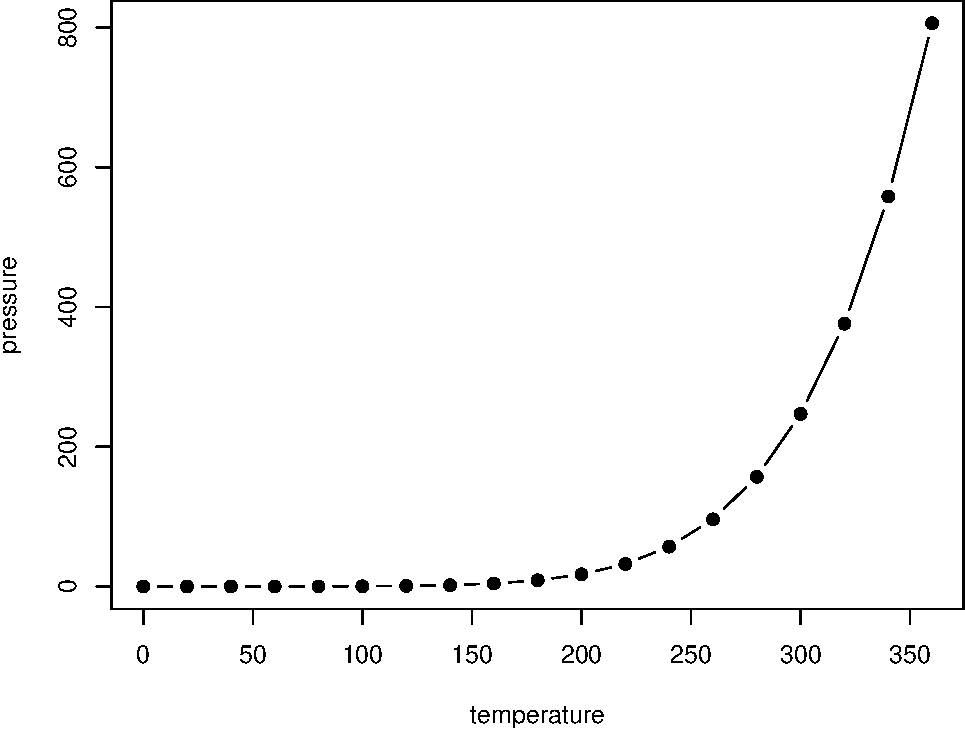
\includegraphics[width=0.8\linewidth]{_main_files/figure-latex/nice-fig-1} 

}

\caption{Here is a nice figure!}\label{fig:nice-fig}
\end{figure}

Don't miss Table \ref{tab:nice-tab}.

\begin{Shaded}
\begin{Highlighting}[]
\NormalTok{knitr}\SpecialCharTok{::}\FunctionTok{kable}\NormalTok{(}
  \FunctionTok{head}\NormalTok{(pressure, }\DecValTok{10}\NormalTok{), }\AttributeTok{caption =} \StringTok{\textquotesingle{}Here is a nice table!\textquotesingle{}}\NormalTok{,}
  \AttributeTok{booktabs =} \ConstantTok{TRUE}
\NormalTok{)}
\end{Highlighting}
\end{Shaded}

\begin{table}

\caption{\label{tab:nice-tab}Here is a nice table!}
\centering
\begin{tabular}[t]{rr}
\toprule
temperature & pressure\\
\midrule
0 & 0.0002\\
20 & 0.0012\\
40 & 0.0060\\
60 & 0.0300\\
80 & 0.0900\\
\addlinespace
100 & 0.2700\\
120 & 0.7500\\
140 & 1.8500\\
160 & 4.2000\\
180 & 8.8000\\
\bottomrule
\end{tabular}
\end{table}

\hypertarget{parts}{%
\chapter{Parts}\label{parts}}

You can add parts to organize one or more book chapters together. Parts can be inserted at the top of an .Rmd file, before the first-level chapter heading in that same file.

Add a numbered part: \texttt{\#\ (PART)\ Act\ one\ \{-\}} (followed by \texttt{\#\ A\ chapter})

Add an unnumbered part: \texttt{\#\ (PART\textbackslash{}*)\ Act\ one\ \{-\}} (followed by \texttt{\#\ A\ chapter})

Add an appendix as a special kind of un-numbered part: \texttt{\#\ (APPENDIX)\ Other\ stuff\ \{-\}} (followed by \texttt{\#\ A\ chapter}). Chapters in an appendix are prepended with letters instead of numbers.

\hypertarget{footnotes-and-citations}{%
\chapter{Footnotes and citations}\label{footnotes-and-citations}}

\hypertarget{footnotes}{%
\section{Footnotes}\label{footnotes}}

Footnotes are put inside the square brackets after a caret \texttt{\^{}{[}{]}}. Like this one \footnote{This is a footnote.}.

\hypertarget{citations}{%
\section{Citations}\label{citations}}

Reference items in your bibliography file(s) using \texttt{@key}.

For example, we are using the \textbf{bookdown} package \citep{R-bookdown} (check out the last code chunk in index.Rmd to see how this citation key was added) in this sample book, which was built on top of R Markdown and \textbf{knitr} \citep{xie2015} (this citation was added manually in an external file book.bib).
Note that the \texttt{.bib} files need to be listed in the index.Rmd with the YAML \texttt{bibliography} key.

The RStudio Visual Markdown Editor can also make it easier to insert citations: \url{https://rstudio.github.io/visual-markdown-editing/\#/citations}

\hypertarget{blocks}{%
\chapter{Blocks}\label{blocks}}

\hypertarget{equations}{%
\section{Equations}\label{equations}}

Here is an equation.

\begin{equation} 
  f\left(k\right) = \binom{n}{k} p^k\left(1-p\right)^{n-k}
  \label{eq:binom}
\end{equation}

You may refer to using \texttt{\textbackslash{}@ref(eq:binom)}, like see Equation \eqref{eq:binom}.

\hypertarget{theorems-and-proofs}{%
\section{Theorems and proofs}\label{theorems-and-proofs}}

Labeled theorems can be referenced in text using \texttt{\textbackslash{}@ref(thm:tri)}, for example, check out this smart theorem \ref{thm:tri}.

\begin{theorem}
\protect\hypertarget{thm:tri}{}\label{thm:tri}For a right triangle, if \(c\) denotes the \emph{length} of the hypotenuse
and \(a\) and \(b\) denote the lengths of the \textbf{other} two sides, we have
\[a^2 + b^2 = c^2\]
\end{theorem}

Read more here \url{https://bookdown.org/yihui/bookdown/markdown-extensions-by-bookdown.html}.

\hypertarget{callout-blocks}{%
\section{Callout blocks}\label{callout-blocks}}

The R Markdown Cookbook provides more help on how to use custom blocks to design your own callouts: \url{https://bookdown.org/yihui/rmarkdown-cookbook/custom-blocks.html}

\hypertarget{sharing-your-book}{%
\chapter{Sharing your book}\label{sharing-your-book}}

\hypertarget{publishing}{%
\section{Publishing}\label{publishing}}

HTML books can be published online, see: \url{https://bookdown.org/yihui/bookdown/publishing.html}

\hypertarget{pages}{%
\section{404 pages}\label{pages}}

By default, users will be directed to a 404 page if they try to access a webpage that cannot be found. If you'd like to customize your 404 page instead of using the default, you may add either a \texttt{\_404.Rmd} or \texttt{\_404.md} file to your project root and use code and/or Markdown syntax.

\hypertarget{metadata-for-sharing}{%
\section{Metadata for sharing}\label{metadata-for-sharing}}

Bookdown HTML books will provide HTML metadata for social sharing on platforms like Twitter, Facebook, and LinkedIn, using information you provide in the \texttt{index.Rmd} YAML. To setup, set the \texttt{url} for your book and the path to your \texttt{cover-image} file. Your book's \texttt{title} and \texttt{description} are also used.

This \texttt{gitbook} uses the same social sharing data across all chapters in your book- all links shared will look the same.

Specify your book's source repository on GitHub using the \texttt{edit} key under the configuration options in the \texttt{\_output.yml} file, which allows users to suggest an edit by linking to a chapter's source file.

Read more about the features of this output format here:

\url{https://pkgs.rstudio.com/bookdown/reference/gitbook.html}

Or use:

\begin{Shaded}
\begin{Highlighting}[]
\NormalTok{?bookdown}\SpecialCharTok{::}\NormalTok{gitbook}
\end{Highlighting}
\end{Shaded}


\end{document}
